\chapter{Introduzione al Machine Learning}\label{ch-01}

La prima lezione ha un doppio scopo: motivare lo studio del
\textbf{Machine Learning} (ML, in italiano \emph{apprendimento
automatico}) collocandolo nel panorama dell'informatica e
dell'intelligenza artificiale, e fornire le informazioni pratiche sul
corso (prerequisiti, struttura, esame, materiale). In chiusura vengono
richiamati i concetti matematici di base che serviranno per tutto il
corso.

\section{Che cos'è il Machine
Learning}\label{che-cosuxe8-il-machine-learning}

\subsection{L'apprendimento come principio
universale}\label{lapprendimento-come-principio-universale}

L'apprendimento è un principio che accomuna esseri viventi, società e
--- oggi --- macchine. Come osservano Poggio e Shelton (\emph{AI
Magazine}, 1999), \emph{il problema dell'apprendimento è probabilmente
il cuore stesso del problema dell'intelligenza, sia biologica che
artificiale}. Capire come si impara significa quindi capire una parte
fondamentale di cosa vuol dire essere intelligenti.

\begin{boxdefinition}{Machine Learning}

Il \textbf{Machine Learning} è un'area teorica e applicativa
dell'informatica che unisce due obiettivi: quello dell'intelligenza
artificiale di costruire \textbf{computer capaci di apprendere}, e
quello di disporre di \textbf{strumenti adattivi e statistici potenti},
con fondamenti rigorosi nelle scienze computazionali. Operativamente, è
l'apprendimento automatico, da parte di un sistema, a partire
dall'\textbf{esperienza} (un insieme di esempi), finalizzato a risolvere
un compito computazionale.

\end{boxdefinition}

\subsection{Perché far apprendere le macchine: lusso o
necessità?}\label{perchuxe9-far-apprendere-le-macchine-lusso-o-necessituxe0}

Il ML non è un vezzo tecnologico ma una \textbf{necessità}, per due
ragioni principali:

\begin{enumerate}
\def\labelenumi{\arabic{enumi}.}
\tightlist
\item
  \textbf{Disponibilità crescente di dati empirici} e bisogno di
  analizzarli. La scienza stessa sta cambiando paradigma verso un
  approccio \emph{data-driven}, in cui la conoscenza si estrae dai dati;
  il ML ha un ruolo centrale e metodologico in questo cambiamento.
\item
  \textbf{È difficile programmare esplicitamente l'adattività e
  l'intelligenza}. Già Alan Turing lo aveva intuito: per molti compiti
  scrivere a mano le regole è impraticabile, e l'apprendimento diventa
  l'unica strada per dotare i sistemi di comportamenti intelligenti.
\end{enumerate}

La combinazione di \textbf{grandi quantità di dati}, \textbf{potenza di
calcolo} (HPC, GPU) e \textbf{flessibilità dei modelli di ML} ha aperto
una nuova era dell'intelligenza artificiale.

\subsection{Quando serve il ML}\label{quando-serve-il-ml}

Il ML è la scelta giusta quando per un problema c'è \textbf{poca o
nessuna conoscenza a priori} (non sappiamo scrivere le regole della
soluzione), ma è relativamente \textbf{facile disporre di esperienza},
cioè di dati di cui conosciamo il risultato corretto. Esempi classici
sono la classificazione delle email come \emph{spam}, il riconoscimento
di caratteri, volti o parlato.

\begin{boxexample}{Riconoscimento di cifre scritte a mano}

Ogni cifra è un'immagine di \(8 \times 8\) pixel. Scrivere a mano le
regole che distinguono un ``3'' da un ``8'' per tutte le possibili
calligrafie è di fatto impossibile. Si raccolgono invece molti esempi di
cifre già etichettate e si lascia che il sistema \textbf{apprenda un
classificatore} \(f\) che associa a ogni immagine la classe corretta
(\(0, 1, \dots, 9\)).

\end{boxexample}

\begin{figure}[htbp]
\centering
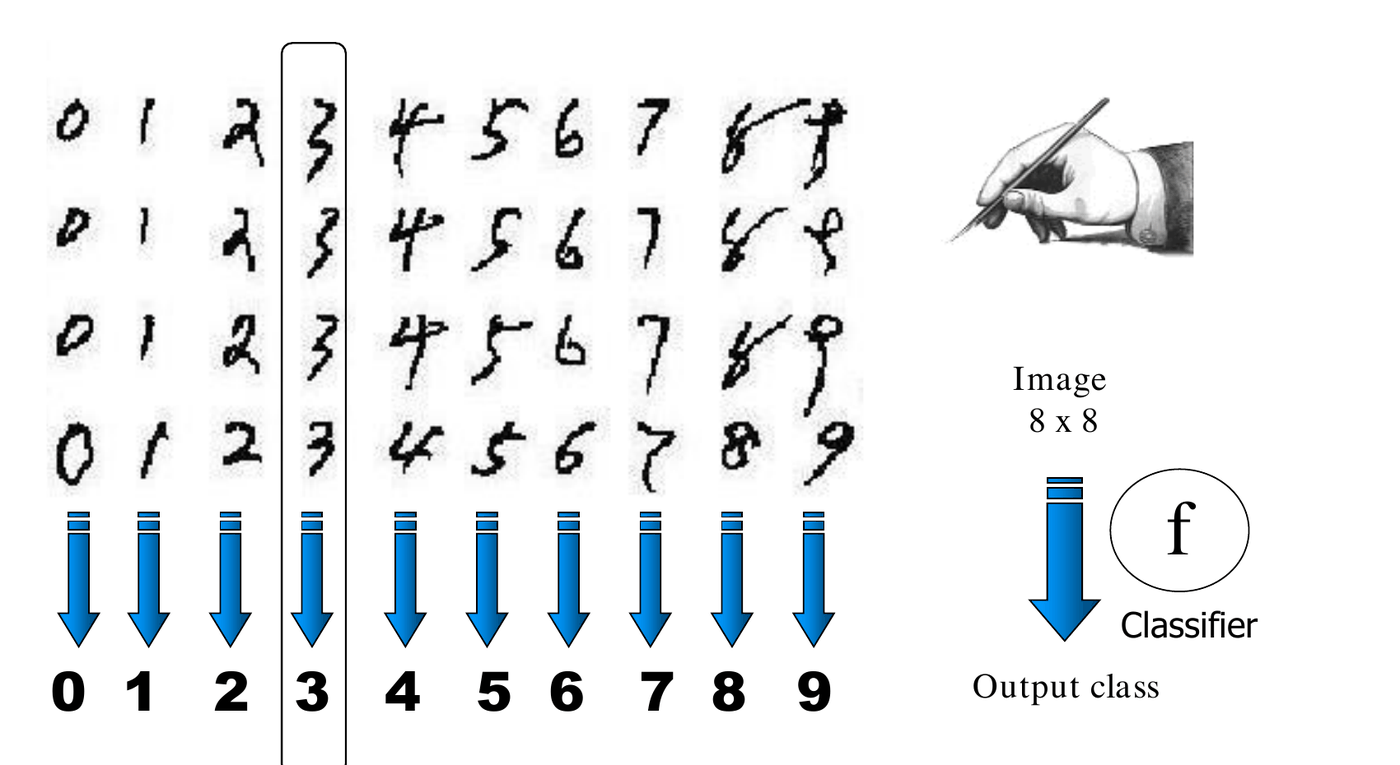
\includegraphics[width=0.80\linewidth,height=0.42\textheight,keepaspectratio]{images/01-intro_cifre-manoscritte.png}
\caption{Riconoscimento di cifre manoscritte: il classificatore \(f\) mappa
un'immagine 8×8 nella classe di output.}
\end{figure}

\subsection{Aree applicative}\label{aree-applicative}

Il ML è ormai pervasivo nei sistemi reali (dall'OCR alle interfacce
uomo-macchina, ai motori di ricerca) ed è il nucleo di un'area
interdisciplinare che dagli anni '80 comprende:

\begin{itemize}
\tightlist
\item
  \textbf{Pattern Recognition} (riconoscimento di volti e parlato),
  \textbf{Computer Vision}, \textbf{Natural Language Processing} (dalla
  classificazione di testi all'elaborazione del parlato fino all'AI
  generativa);
\item
  \textbf{Robotica}, sistemi e filtri adattivi, reti di sensori
  intelligenti, componenti personalizzati;
\item
  \textbf{Knowledge Discovery e Data Mining}, Information Retrieval,
  analisi di dati complessi (medicina, biologia, chimica, web,
  marketing), previsioni finanziarie.
\end{itemize}

In alcuni campi --- NLP, Pattern Recognition, Computer Vision ---
l'impatto è stato rivoluzionario, tanto da parlare di una ``nuova AI''.

\subsection{Alcuni successi recenti}\label{alcuni-successi-recenti}

Il professore mostra alcuni risultati emblematici:

\begin{itemize}
\tightlist
\item
  \textbf{Riconoscimento facciale (DeepFace, CVPR 2014)}: combinando
  reti neurali profonde e altre tecniche di ML, addestrato su quattro
  milioni di immagini di oltre 4000 persone, il sistema stabilisce se
  due foto ritraggono la stessa persona con un'accuratezza del 97,25\%,
  appena sotto quella umana (97,53\%).
\item
  \textbf{AlphaGo (DeepMind, marzo 2016)}: sconfigge il campione
  mondiale di Go.
\item
  \textbf{Medicina}: una rete neurale profonda per la classificazione
  dei tumori della pelle, addestrata su 130.000 casi (più di quanti un
  medico ne veda ``in molte vite''), raggiunge l'accuratezza di
  dermatologi certificati (\emph{Nature}, 2017). Al CIML di Pisa, il
  progetto BrAID applica l'AI alla diagnosi della sindrome di Brugada.
\item
  \textbf{Traduzione automatica}: Google Neural Machine Translation (dal
  2016) e DeepL (dal 2017), interamente basati su reti neurali.
\item
  \textbf{Large Language Models e AI generativa}: ChatGPT (OpenAI,
  novembre 2022), Bard/LaMDA (Google), modelli open source come Dolly, e
  sistemi che generano immagini (Stable Diffusion), video, musica.
\item
  Guida autonoma, analisi di dati da sensori, IoT.
\end{itemize}

Il ML fornisce la base teorica e metodologica della cosiddetta
\emph{rivoluzione dell'AI}, con enormi investimenti industriali. Viene
considerato una \textbf{GPT} (\emph{General-Purpose Technology}): una
tecnologia capace di trasformare profondamente le strutture economiche e
sociali preesistenti. La figura del ``\emph{ML scientist}'' è tra le più
richieste nel mercato del lavoro.

\begin{boxnote}{Premio Turing 2018}

Il 27 marzo 2019 l'ACM ha assegnato il Premio Turing (il ``Nobel
dell'informatica'') a \textbf{Yoshua Bengio, Geoffrey Hinton e Yann
LeCun} ``per le scoperte concettuali e ingegneristiche che hanno reso le
reti neurali profonde una componente critica dell'informatica''.

\end{boxnote}

\begin{boxnote}{Premi Nobel 2024}

Nel 2024 il ML è arrivato anche ai Nobel: - \textbf{Fisica}: a
\textbf{John Hopfield} e \textbf{Geoffrey Hinton} per le scoperte e
invenzioni fondamentali che permettono il machine learning con le reti
neurali artificiali (la rete di Hopfield come memoria associativa, la
macchina di Boltzmann). - \textbf{Chimica}: a \textbf{Demis Hassabis} e
\textbf{John Jumper} (Google DeepMind) per la predizione della struttura
delle proteine con \textbf{AlphaFold}, e a \textbf{David Baker} per la
progettazione computazionale di proteine. Hassabis: \emph{``Ho sempre
pensato che, se riuscissimo a costruire l'AI nel modo giusto, potrebbe
essere lo strumento definitivo per aiutare gli scienziati a esplorare
l'universo che ci circonda.''}

\end{boxnote}

\subsection{Lo scopo ultimo}\label{lo-scopo-ultimo}

Tutto ciò che è potente può essere pericoloso se usato male, ma lo scopo
ultimo di AI e ML è \textbf{portare benefici alle persone} risolvendo
problemi grandi e piccoli, \textbf{accelerare il progresso umano} e
fornire intelligenza a ogni altro campo scientifico: aumentare le nostre
capacità, esaltando la nostra umanità (P. Domingos, \emph{Scientific
American}, 2018).

\section{Perché studiare il Machine
Learning}\label{perchuxe9-studiare-il-machine-learning}

Nel percorso di laurea magistrale il ML serve a:

\begin{itemize}
\tightlist
\item
  conoscere i \textbf{principi di base dei processi di apprendimento},
  dal punto di vista computazionale;
\item
  conoscere \textbf{nuovi paradigmi di calcolo}, come le \textbf{reti
  neurali}: studiate come paradigma computazionale dagli anni `40 con
  ispirazione neurobiologica, oggi sono un insieme di modelli potenti
  per l'\textbf{approssimazione di funzioni} con capacità predittive,
  supportati da una solida teoria (la \emph{learning theory}), e sono
  alla base del \textbf{Deep Learning};
\item
  saper \textbf{applicare questi modelli con rigore};
\item
  avere le basi per tutti i corsi successivi di AI.
\end{itemize}

\subsection{Il ML moderno}\label{il-ml-moderno}

Il ML è passato dall'essere una \textbf{collezione di metodi euristici}
(trucchi provenienti da biologia, statistica, reti neurali, logica
fuzzy\ldots) alla costruzione di \textbf{quadri concettuali generali}. È
emersa una nuova comprensione dei principi che governano i processi di
apprendimento, con tre conseguenze importanti:

\begin{itemize}
\tightlist
\item
  esprimere modelli diversi in ``linguaggi'' matematici o informatici
  diversi \textbf{non cambia i principi};
\item
  campi applicativi diversi \textbf{non cambiano i principi};
\item
  nuovi avanzamenti tecnologici \textbf{non cambiano i principi}.
\end{itemize}

\begin{boxtip}{Il filo conduttore del corso}

Il ``Machine Learning'' in senso proprio è il \textbf{nucleo di principi
e metodi} per costruire modelli computazionali flessibili e potenti a
partire dai dati. I singoli modelli cambiano, i principi restano: è
questo che conviene imparare davvero.

\end{boxtip}

\subsection{Tre punti di vista sul ML}\label{tre-punti-di-vista-sul-ml}

\begin{enumerate}
\def\labelenumi{\arabic{enumi}.}
\tightlist
\item
  \textbf{Come metodologia di AI} → costruire sistemi adattivi e
  intelligenti.
\item
  \textbf{Come apprendimento statistico} (inferenza di ipotesi secondo
  principi matematici) → costruire potenti sistemi predittivi per
  l'analisi intelligente dei dati.
\item
  \textbf{Come metodo informatico per aree applicative innovative} →
  usare i modelli come strumenti per problemi complessi e
  interdisciplinari.
\end{enumerate}

Il corso li considera tutti, con un \textbf{approccio critico}: dei vari
metodi si discutono i limiti e l'appropriatezza d'uso, con attenzione ai
principi sottostanti. Gli obiettivi pratici sono due: imparare a
\textbf{sviluppare nuovi modelli} di ML e imparare ad \textbf{applicare
le metodologie allo stato dell'arte} a problemi di altri campi.

\section{Informazioni sul corso}\label{informazioni-sul-corso}

\subsection{Prerequisiti e obiettivi}\label{prerequisiti-e-obiettivi}

Nessun corso è strettamente necessario: si parte da zero. Servono però
le basi tipiche di una laurea triennale scientifica: \textbf{analisi
matematica} (funzioni, calcolo differenziale), \textbf{notazione e
calcolo matriciale}, \textbf{elementi di probabilità e statistica},
\textbf{algoritmi}.

Il corso introduce i principi e l'analisi critica dei principali
paradigmi (modelli e algoritmi, con focus sulle reti neurali) per
l'apprendimento dai dati. I concetti vengono introdotti
progressivamente, dagli approcci più semplici fino ai modelli allo stato
dell'arte, all'interno del quadro concettuale del ML moderno:
l'\textbf{apprendimento di funzioni a partire da esempi}. L'attenzione è
su:

\begin{itemize}
\tightlist
\item
  analisi critica delle caratteristiche per la progettazione e l'uso del
  ML;
\item
  \textbf{valutazione sperimentale rigorosa}: c'è una grande differenza
  tra \emph{usare} strumenti di ML e usarli \emph{correttamente};
\item
  aspetti computazionali dei sistemi di apprendimento.
\end{itemize}

\subsection{Struttura del corso}\label{struttura-del-corso}

Il corso ha una struttura forte: si parte dai modelli semplici per
arrivare allo stato dell'arte, e i concetti fondamentali vengono
introdotti attraverso modelli diversi. Il consiglio pratico è duplice:
(1) studiare i singoli metodi, (2) cercare le \textbf{connessioni e i
confronti} tra di essi, così da astrarre i concetti. Il filo rosso è la
comprensione del rapporto tra \textbf{flessibilità del modello} e
\textbf{controllo della complessità}, concetto fondamentale per la
capacità di \textbf{generalizzazione}.

\begin{figure}[htbp]
\centering
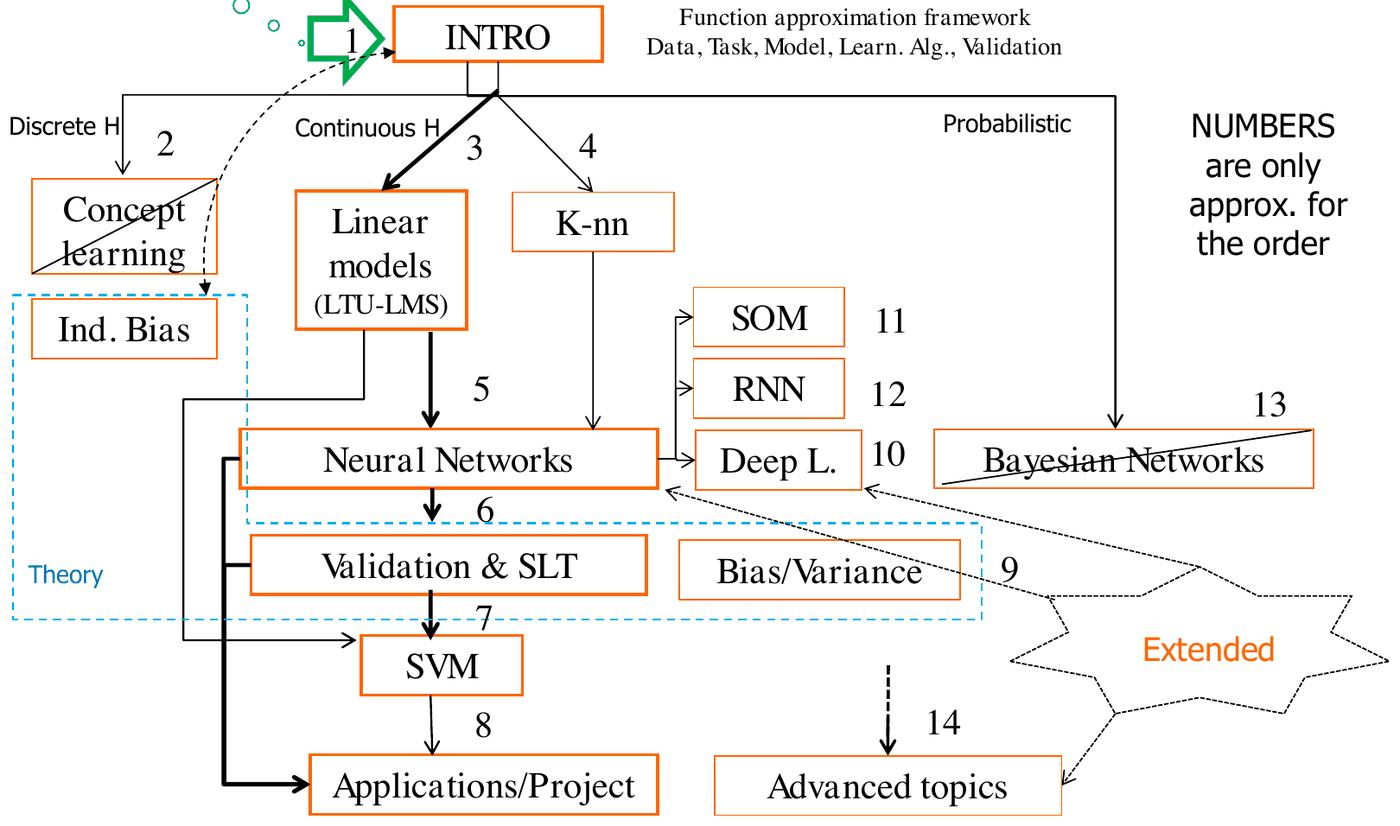
\includegraphics[width=0.93\linewidth,height=0.42\textheight,keepaspectratio]{images/01-intro_struttura-corso.png}
\caption{La mappa del corso. I numeri indicano approssimativamente l'ordine delle
lezioni; il riquadro tratteggiato ``Theory'' raccoglie le parti
teoriche.}
\end{figure}

La mappa non è solo un ordine delle lezioni: descrive il percorso. Si
introducono dei \textbf{``mattoni''} (concetti e modelli intermedi) che
poi vengono composti per costruire i modelli di ML --- ad esempio le
reti neurali si costruiscono dai modelli lineari, e un sistema di ML
completo si costruisce dalle tecniche di validazione. Per questo i
modelli intermedi vanno visti come pezzi di un puzzle che si ricompone
alla fine.

\begin{boxnote}{Ordine delle lezioni secondo la mappa}

\begin{enumerate}
\def\labelenumi{\arabic{enumi}.}
\tightlist
\item
  Introduzione (dati, task, modello, algoritmo di apprendimento,
  validazione) --- nel quadro dell'\textbf{approssimazione di funzioni}.
\item
  Concept learning e bias induttivo (spazio delle ipotesi discreto).
\item
  Modelli lineari (LTU, LMS) (spazio delle ipotesi continuo).
\item
  K-nearest neighbors.
\item
  Reti neurali.
\item
  Validazione e Statistical Learning Theory.
\item
  Support Vector Machines.
\item
  Applicazioni e progetto.
\item
  Bias/Varianza.
\item
  Deep Learning (e, in estensione, SOM, RNN). 11--14. SOM, RNN, (Reti
  Bayesiane --- rimosse dal programma), argomenti avanzati (dati
  strutturati).
\end{enumerate}

\end{boxnote}

La densità del corso non è uniforme: l'introduzione è lenta e
``morbida'', il nucleo (reti neurali, SVM, validazione) è denso e
consequenziale, la parte avanzata è veloce ma meno densa. Il progetto
(opzionale) viene annunciato circa a metà corso.

\subsection{Organizzazione pratica}\label{organizzazione-pratica}

\begin{itemize}
\tightlist
\item
  \textbf{Docente}: Prof.~Alessio Micheli (Dipartimento di Informatica),
  professore ordinario, responsabile del gruppo CIML
  (\emph{Computational Intelligence \& Machine Learning}) con oltre 25
  anni di ricerca in ML/AI, \textbf{presidente della European Neural
  Network Society} (conferenza annuale ICANN), co-fondatore della IEEE
  Task Force on Reservoir Computing, associate editor di IEEE TNNLS e
  \emph{Neural Networks}. Obiettivo del corso: introdurre in 3 mesi al
  ML attuale, ripercorrendone anche le basi e la storia.
\item
  \textbf{Lezioni} (a.a. 2026/27): martedì, mercoledì e giovedì 16--18,
  Aula E. L'inizio è puntuale per poter fare una pausa.
\item
  \textbf{Q\&A} con il docente: il martedì dopo la lezione (tempo
  facoltativo, non parte della lezione) più alcune lezioni speciali di
  Q\&A. Per domande personali si scrive una mail con il tag
  \textbf{{[}ML-26-Q{]}} nell'oggetto (obbligatorio).
\item
  \textbf{Comunicazioni}: tramite Teams e/o le news di Moodle. Le
  \textbf{registrazioni} delle lezioni sono su Teams (scheda
  \emph{Shared} → \emph{Recordings}); le lezioni ufficiali sono solo in
  presenza, lo streaming è informale e senza interazione garantita.
\item
  \textbf{Recuperi}: il lunedì pomeriggio (annunciati quando servono) e
  nel periodo di recupero dal 9 al 18 dicembre 2026 (da considerare
  prima di programmare le vacanze di Natale). Le lezioni del 15--17
  settembre 2026 non si sono tenute e saranno recuperate.
\end{itemize}

\begin{boxnote}{Chi arriva in ritardo al corso}

Tutte le informazioni sono sul \textbf{Moodle} del corso
(elearning.di.unipi.it, con iscrizione autonoma tramite account Unipi):
slide, bibliografia e sezione \textbf{FAQ}. Conviene usare anche Teams
(news e registrazioni) e gli appunti dei colleghi. Progetto e test di
esercizio \textbf{non sono obbligatori} per l'esame. Non chiedere al
docente ciò che è già nelle FAQ o nella prima lezione.

\end{boxnote}

\subsection{Esame}\label{esame}

\begin{boxwarning}{Regole aggiornate (a.a. 2026/27)}

Le modalità d'esame sono cambiate rispetto agli anni precedenti: il
\textbf{progetto non è più obbligatorio} e l'esame si basa su uno
\textbf{scritto obbligatorio}, con orale solo se necessario.

\end{boxwarning}

L'esame si articola, in ordine cronologico, in quattro fasi.

\textbf{1. Test di esercizio durante il corso (opzionali).} Alla fine di
ogni ciclo di lezioni vengono proposti su Moodle brevi e semplici test
di esercizio. Servono per l'\textbf{autovalutazione} (come esercizi per
casa, con un punteggio che però \textbf{non vale per l'esame}), tengono
al passo con le lezioni e sono una testimonianza della partecipazione
attiva. Hanno una scadenza (tipicamente una settimana), ma se se ne
perde qualcuno si può continuare la serie. Preparano allo scritto, anche
se formato, contenuti e profondità sono diversi. Vengono annunciati solo
in aula e con un breve messaggio su Teams.

\textbf{2. Progetto (opzionale).} Alla fine del corso (dicembre) si può
svolgere un progetto:

\begin{itemize}
\tightlist
\item
  lavoro di gruppo di \textbf{2 studenti}, senza eccezioni;
\item
  contenuto: implementazione, applicazione e/o analisi di un metodo o di
  una tecnica di ML/reti neurali con \textbf{valutazione sperimentale}
  (possibili progetti coordinati con il corso di CM);
\item
  formato: presentazione pubblica di un \textbf{poster} in aula (una
  delle ultime lezioni), più la consegna del materiale sviluppato; è
  previsto un premio per il miglior poster;
\item
  dopo la presentazione si può sostenere l'esame in qualunque sessione,
  ma per discutere il progetto i due membri del gruppo devono fare
  l'esame \textbf{nella stessa sessione}.
\end{itemize}

Il consiglio è di non candidarsi al progetto prima di aver studiato a
fondo i contenuti del corso. I dettagli verranno dati in una lezione
dedicata.

\textbf{3. Scritto (obbligatorio).} Si svolge dopo il corso, nelle
sessioni d'esame (da gennaio e febbraio):

\begin{itemize}
\tightlist
\item
  è obbligatorio \textbf{iscriversi} all'appello su esami.unipi.it entro
  la scadenza (verificarla con largo anticipo) e cancellare l'iscrizione
  se si decide di non partecipare;
\item
  si svolge \textbf{solo in presenza}, in aula, nella data, ora e aula
  indicate su esami.unipi.it; non presentarsi equivale a ritirarsi da
  quella sessione;
\item
  le domande vanno risposte su \textbf{fogli prestampati} con spazio per
  la risposta libera; bisogna portare penna o matita;
\item
  le risposte richiedono \textbf{equazioni, disegni e/o parti
  descrittive} (quiz e domande aperte);
\item
  non si può usare alcun materiale del corso o esterno, né alcun ausilio
  elettronico (assistenti virtuali, chatbot\ldots): è vietato l'uso di
  qualunque dispositivo (portatili, smartphone, braccialetti smart,
  auricolari, occhiali smart\ldots), pena l'esclusione.
\end{itemize}

\textbf{4. Orale (solo se necessario) e verbalizzazione.} Per accedere
all'orale serve un livello sufficiente nello scritto (la lista degli
ammessi è comunicata su Moodle). L'orale si tiene nella stessa sessione
dello scritto, in presenza, tipicamente nello studio del docente: nei
giorni successivi alla correzione il docente assegna uno slot a ogni
studente o gruppo. Se serve (in base all'esito dello scritto), l'orale è
un colloquio su \textbf{tutto il programma} e può includere la
discussione dello scritto e del progetto. Esigenze particolari
(priorità, impossibilità di essere in presenza\ldots) si valutano caso
per caso su richiesta.

\begin{boxabstract}{Riepilogo delle regole}

La valutazione tiene conto di: \textbf{risultato dello scritto} +
partecipazione attiva (inclusi i test durante il corso) + attività extra
facoltative (progetto, presentazioni volontarie a fine corso) +
eventuale orale completo, se richiesto dal docente.

\begin{itemize}
\tightlist
\item
  Scritto \textbf{sufficiente} → in uno slot pochi giorni dopo:
  eventuale orale e \textbf{proposta di voto} → se accettata,
  verbalizzazione.
\item
  Scritto \textbf{insufficiente} o voto non accettato → si ripete in una
  sessione successiva, a scelta tra le molte dell'anno.
\end{itemize}

Completare l'80\% dei test online e un progetto molto buono possono dare
un \textbf{piccolo bonus} (se lo scritto è già sufficiente o buono), ma
\textbf{non sono necessari} né per sostenere l'esame né per ottenere il
voto massimo. L'indicatore chiave è la \textbf{conoscenza finale del ML
e la sua profondità}.

\end{boxabstract}

\begin{boxtip}{I consigli del professore}

\begin{itemize}
\tightlist
\item
  Seguire le lezioni usando le slide come guida e studiare
  progressivamente durante il corso; le lezioni di Q\&A sono un forum di
  discussione: è una classe, non un insieme di registrazioni.
\item
  Prima \textbf{studiare i contenuti} del corso, poi dedicarsi al
  progetto: aumenta sia l'efficacia sia l'efficienza del lavoro.
\item
  Se qualcosa non è chiaro: niente panico, chiedere al docente (Q\&A),
  collaborare con i colleghi, usare libri e articoli (bibliografia e
  ricerca personale) e i supporti del corso. Il ML è un campo in
  continua evoluzione: va studiato!
\end{itemize}

\end{boxtip}

\subsection{Materiale e bibliografia}\label{materiale-e-bibliografia}

Il riferimento principale sono le slide del corso (su Moodle, spesso
pubblicate in anticipo; attenzione a usare l'ultima versione dei file
\texttt{ML-26…-v*}), che però vanno integrate con i propri appunti (le
slide da sole possono non bastare a ricostruire il filo della lezione) e
con i libri. Il docente è disponibile a condividere su Moodle gli
appunti degli studenti. I testi principali sono:

\begin{itemize}
\tightlist
\item
  S. Haykin, \emph{Neural Networks and Learning Machines}, Prentice
  Hall, 3ª ed., 2008;
\item
  T. M. Mitchell, \emph{Machine Learning}, McGraw-Hill, 1997;
\item
  I. Goodfellow, Y. Bengio, A. Courville, \emph{Deep Learning}, MIT
  Press, 2016 (gratuito online).
\end{itemize}

Altri riferimenti utili: Russell--Norvig (\emph{AIMA}),
Hastie--Tibshirani--Friedman (\emph{The Elements of Statistical
Learning}, copia gratuita online), Cherkassky--Mulier, Bishop
(\emph{Pattern Recognition and Machine Learning}, ora \textbf{gratuito}
dal sito dell'editore; e \emph{Neural Networks for Pattern
Recognition}), Duda--Hart--Stork, Shalev-Shwartz--Ben-David
(\emph{Understanding Machine Learning}, gratuito online).

Per le \textbf{librerie software}: F. Chollet, \emph{Deep Learning with
Python}; A. Géron, \emph{Hands-on Machine Learning with Scikit-Learn,
Keras \& TensorFlow}; A. Zhang, Z. Lipton, M. Li, A. Smola, \emph{Dive
into Deep Learning} (Cambridge University Press, 2023, gratuito online,
con esempi in PyTorch, NumPy/MXNet, JAX e TensorFlow). Le librerie
principali verranno introdotte più avanti dall'assistente del corso.
Attenzione: esistono moltissimi libri e blog tecnici, bisogna badare
alla qualità scientifica.

\begin{boxnote}{Supporti al corso}

\begin{itemize}
\tightlist
\item
  Un \textbf{assistente del corso} per aiutare nello sviluppo del
  progetto (da confermare).
\item
  Un \textbf{chatbot tutor} (basato su ChatGPT), sperimentale, per il
  corso ML 2026: serve a chiarire dubbi, approfondire concetti e avere
  indicazioni su slide, definizioni ed esercizi, sempre sulla base dei
  materiali ufficiali del corso. Dettagli e link saranno pubblicati
  nelle news di Moodle.
\end{itemize}

\end{boxnote}

In parallelo è molto utile il corso di \textbf{Computational Mathematics
for Learning and Data Analysis} (CM), che fornisce le basi matematiche
profonde dei metodi di apprendimento (non è però obbligatorio per
seguire ML).

\section{Richiami matematici}\label{richiami-matematici}

Per seguire il corso servono alcuni concetti di base: calcolo in più
variabili (derivate parziali, gradiente), probabilità (densità, media,
varianza, normale, probabilità condizionate e congiunte), calcolo
matriciale (prodotto scalare, inversa, norme). Argomenti come il
problema dei minimi quadrati lineari con la SVD e i moltiplicatori di
Lagrange possono essere approfonditi in parallelo. Riferimenti
consigliati: appendice A di AIMA, capitoli 2--4 del \emph{Deep Learning
book}, e \emph{Mathematics for Machine Learning} (2020).

La notazione usata è: \(x\) scalare, \(\mathbf{x}\) vettore, \(X\)
matrice.

\subsection{Prodotto scalare e norme}\label{prodotto-scalare-e-norme}

\begin{boxdefinition}{Prodotto scalare (\emph{inner/dot product})}

\[
\mathbf{a} \cdot \mathbf{b} = a_1 b_1 + a_2 b_2 + \dots + a_n b_n = \sum_{i=1}^{n} a_i b_i = |\mathbf{a}|\,|\mathbf{b}| \cos\theta
\]

Notazioni equivalenti:
\(\mathbf{a}\cdot\mathbf{b} = \mathbf{a}^T\mathbf{b} = \mathbf{a}^t\mathbf{b} = \langle \mathbf{a}, \mathbf{b}\rangle\),
e anche solo \(\mathbf{ab}\) se il contesto è chiaro.

\end{boxdefinition}

La relazione con il coseno dà l'intuizione geometrica: il prodotto
scalare misura \textbf{quanto due vettori puntano nella stessa
direzione}. È massimo quando sono paralleli, nullo quando sono
ortogonali, negativo quando puntano in versi opposti. Questa lettura
tornerà di continuo (ad esempio nei modelli lineari, dove
\(\mathbf{w}^T\mathbf{x}\) misura l'\,``allineamento'' dell'input con i
pesi).

La \textbf{norma euclidea} (modulo, lunghezza) di un vettore è \[
\|\mathbf{x}\|_2 = \sqrt{\mathbf{x}^T\mathbf{x}} = \sqrt{\sum_i x_i^2} = d(\mathbf{x}, \mathbf{0}),
\] spesso scritta semplicemente \(\|\mathbf{x}\|\) o \(|\mathbf{x}|\).
Altre norme utili sono la \textbf{norma \(L^1\)},
\(\|\mathbf{x}\|_1 = \sum_i |x_i|\), e la \textbf{norma del massimo},
\(\|\mathbf{x}\|_\infty = \max_i |x_i|\).

Più in generale, un \textbf{prodotto interno}
\(\langle \cdot,\cdot \rangle\) è una forma bilineare simmetrica che
associa a una coppia di vettori uno scalare: \[
\langle v, w\rangle = \langle w, v\rangle, \qquad \langle v+w, u\rangle = \langle v,u\rangle + \langle w,u\rangle, \qquad \langle kv, w\rangle = k\langle v, w\rangle.
\] Vale la \textbf{disuguaglianza di Cauchy-Schwarz}:
\(|\langle x, y\rangle| \le \|x\|\cdot\|y\|\) per ogni \(x, y \in V\).

\begin{boxnote}{Tensori}

Un \textbf{tensore}, nella visione semplificata usata in ML, è un array
multidimensionale di numeri disposti su una griglia regolare con un
numero variabile di assi (ad esempio \(X_{i,j,k}\) ha 3 indici). In ML
si usa soprattutto come comodità di notazione e per ragionare sul
calcolo su GPU; in matematica i tensori hanno proprietà più ricche
(legate ai cambi di base).

\end{boxnote}

\subsection{Derivate parziali e
gradiente}\label{derivate-parziali-e-gradiente}

La \textbf{derivata parziale} generalizza la derivata a funzioni di più
variabili: è la derivata rispetto a una sola variabile tenendo fisse
tutte le altre. Per \(f(x_1, x_2, x_3)\) si calcolano
\(\frac{\partial f}{\partial x_1}\),
\(\frac{\partial f}{\partial x_2}\),
\(\frac{\partial f}{\partial x_3}\).

\begin{boxdefinition}{Gradiente}

Il \textbf{gradiente} di \(f\) è il vettore delle sue derivate parziali:
\[
\nabla f = \operatorname{grad} f = \left( \frac{\partial f}{\partial x_1}, \dots, \frac{\partial f}{\partial x_n} \right) = \sum_{i=1}^{n} \frac{\partial f}{\partial x_i}\, \mathbf{e}_i
\] dove gli \(\mathbf{e}_i\) sono i versori ortogonali lungo le
direzioni coordinate.

\end{boxdefinition}

Il significato geometrico è fondamentale per tutto il corso: in un
punto, il gradiente è un vettore che \textbf{punta nella direzione di
massima pendenza}, e la sua norma indica \textbf{quanto è ripida} la
pendenza. Il gradiente indica quindi dove la funzione cresce più
rapidamente, mentre il suo opposto \(-\nabla f\) indica la direzione in
cui \textbf{decresce} più rapidamente. È esattamente questa l'idea alla
base della \textbf{discesa del gradiente} (\emph{gradient descent}), che
useremo per addestrare i modelli minimizzando una funzione di errore.

\begin{figure}[htbp]
\centering
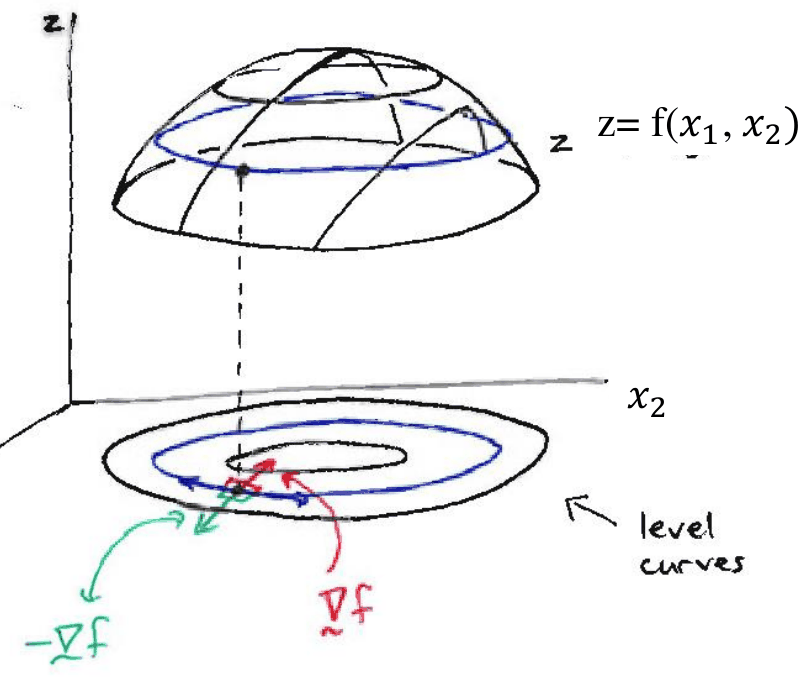
\includegraphics[width=0.47\linewidth,height=0.42\textheight,keepaspectratio]{images/01-intro_gradiente-superficie.png}
\caption{Gradiente su una superficie: \(\nabla f\) punta verso la crescita di
\(f\), \(-\nabla f\) verso la decrescita; entrambi sono perpendicolari
alle curve di livello.}
\end{figure}

Un punto in cui il gradiente è nullo si dice \textbf{punto stazionario}.
Può essere un minimo locale, un massimo locale o un punto di sella: il
gradiente nullo da solo non basta a dire di quale caso si tratta.

\begin{figure}[htbp]
\centering
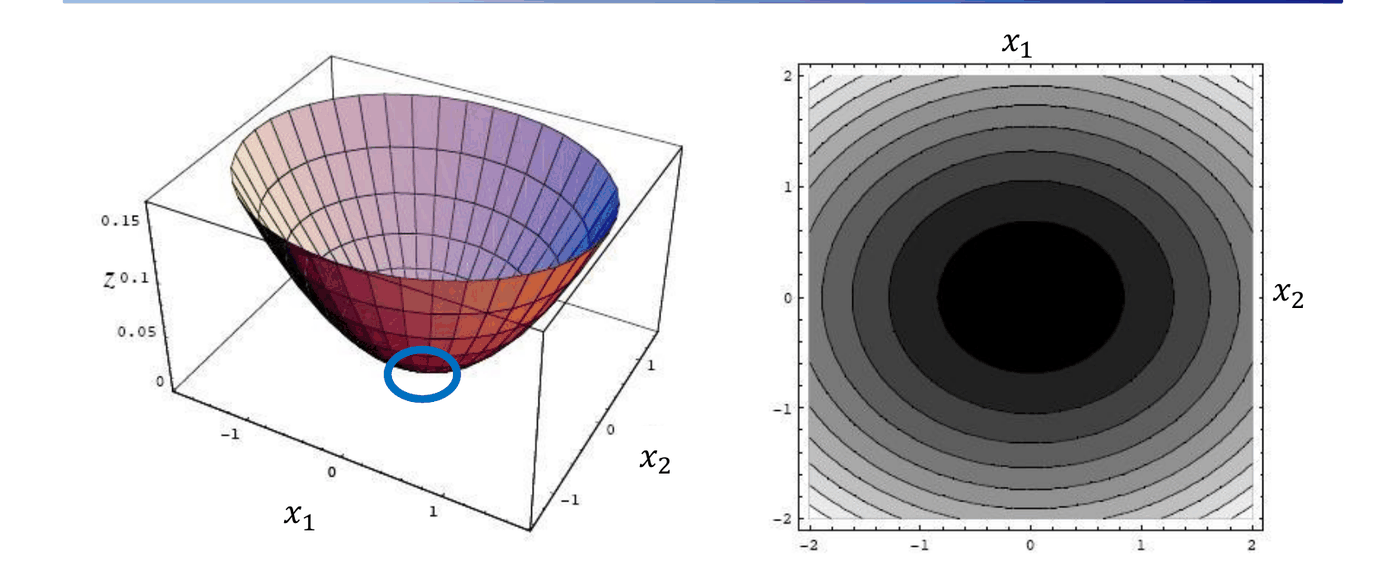
\includegraphics[width=0.80\linewidth,height=0.42\textheight,keepaspectratio]{images/01-intro_minimo-locale.png}
\caption{Un minimo: nel punto più basso del paraboloide il gradiente è zero.}
\end{figure}

\subsection{Densità di probabilità: la
gaussiana}\label{densituxe0-di-probabilituxe0-la-gaussiana}

La \textbf{distribuzione normale} con media \(\mu\) e varianza
\(\sigma^2\) ha densità di probabilità (la ``funzione gaussiana'') \[
f(x) = \frac{1}{\sigma\sqrt{2\pi}}\, e^{-(x-\mu)^2 / (2\sigma^2)}.
\] Con \(\mu = 0\) e \(\sigma^2 = 1\) si ottiene la \textbf{normale
standard}.

\begin{figure}[htbp]
\centering
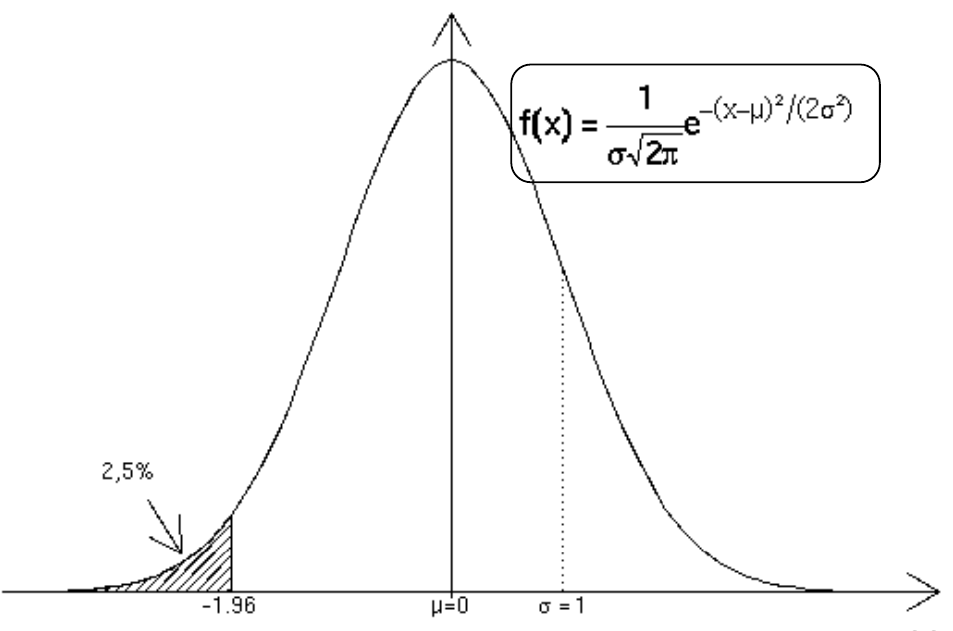
\includegraphics[width=0.57\linewidth,height=0.42\textheight,keepaspectratio]{images/01-intro_gaussiana.png}
\caption{Densità della normale standard: l'area a sinistra di \(-1{,}96\) vale il
2,5\%.}
\end{figure}

\section{Sintesi e prossimi passi}\label{sintesi-e-prossimi-passi}

\begin{boxabstract}{Sintesi}

Il ML è l'apprendimento automatico di un compito a partire da esempi: è
necessario quando i dati abbondano ma le regole esplicite mancano. Il
corso lo affronta come \textbf{approssimazione di funzioni a partire da
esempi}, costruendo i modelli per ``mattoni'' successivi, con attenzione
ai principi (che non cambiano al variare dei modelli) e alla valutazione
rigorosa. Il concetto chiave che attraversa tutto il corso è il
compromesso tra \textbf{flessibilità del modello} e \textbf{controllo
della complessità}, da cui dipende la \textbf{generalizzazione}.

\end{boxabstract}

Le lezioni successive completano l'introduzione: nelle lezioni 2--3 si
vedono l'utilità del ML, l'apprendimento come approssimazione di
funzioni con un esempio guida, e le componenti di progetto di un sistema
di ML (task, spazio delle ipotesi, bias induttivo, funzione di loss,
generalizzazione); nella lezione 4 si approfondiscono generalizzazione e
validazione.

\begin{boxquestion}{Possibili domande d'esame}

\begin{itemize}
\tightlist
\item
  Perché il ML è una necessità e non un lusso? In quali condizioni è
  appropriato usarlo?
\item
  Che cos'è il gradiente e perché \(-\nabla f\) indica la direzione di
  massima decrescita?
\item
  Che cos'è un punto stazionario? È sempre un minimo?
\end{itemize}

\end{boxquestion}
